\subsection{Concept}
A neural network is grown in a \textit{MEA}, short for \textit{micro electrode
 array} which allows the neurons to be interfaced with using electrical stimuli
in order to control a robot as shown in \ref{fig:cyborg_idea}.
Building on the theoretical groundwork described in the background, the neural
network is used as a reservoir which is fed sensory input from a robot.
This system is a \textit{closed loop}, it does not require any outside
intervention such as a human controller using a joystick to operate.
A somewhat subtle but very important consequence of utilizing reservoir
computing is that the neural network does not directly control the robot, it
simply acts as a classifier which responds to the input, and the resulting
dynamics is interpreted by a computer as an action for the robot.
This distinction has little practical consequence for the cyborg, but may offer
a clue into the inner workings of sentience.
\begin{figure}[h!]
    %\centering
    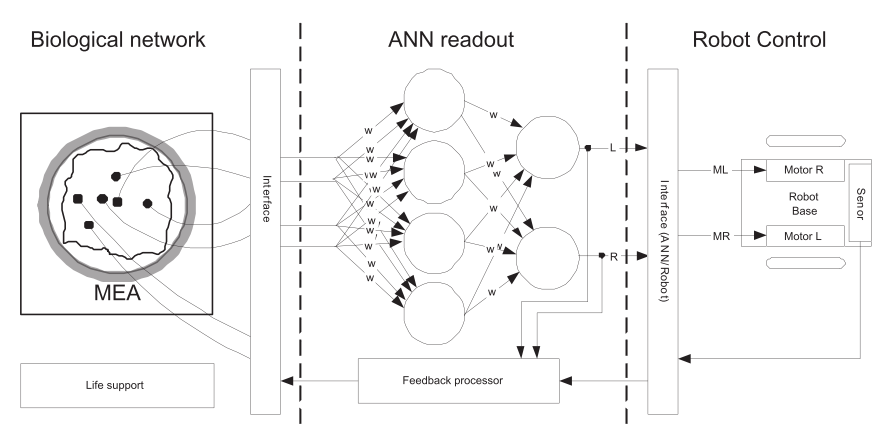
\includegraphics[width=\linewidth]{images/cyborg_overview.png}
    \caption{The gist of it..}
    \label{fig:cyborg_idea}
\end{figure}
\subsection{Platform}
Providing an interface between neurons and a computer allows using neural
network for computation, however it is impractical to move the neural cultures
outside of the laboratory.
The practical, yet thought provoking\footnote{For brevity the
  philosophical implications is left as an exercise to the reader.} solution is
using a TCP/IP network protocol such that the neuron culture may be interfaced with any
robot or simulator without leaving the laboratory.
Similar network architectures have been implemented, in
\cite{li_application_2015} a neuron culture is used to control a simple
wall-avoiding robot as a proof of concept.
In contrast with previous work the robot used in the NTNU cyborg project is a
sophisticated robot which can move by itself, follow a person, take a selfie
with someone and upload it to facebook, and even perform a secret handshake.
By utilizing an already functioning robot as a host the cyborg project can focus
on extending the capabilities of the robot, making it a true hybrid between
digital and cellular computing.
\begin{figure}[h!]
    %\centering
    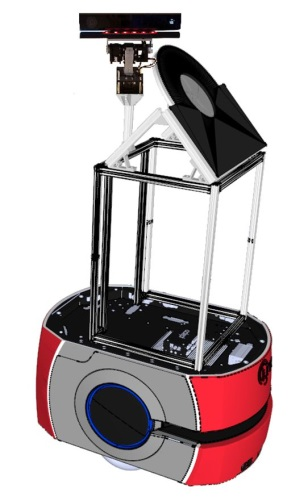
\includegraphics[width=\linewidth]{images/cyborg.jpg}
    \caption{robot render}
    \label{fig:cyborg}
\end{figure}
\subsection{Growing Neurons In Vitro}
The neuron cultures used in the cyborg are being grown in MEAs
at the department of neuroscience.
The MEAs are seeded with neural stem cells of either human or rat origin which
then spontaneously form networks.
At seeding there is no network at all, only a ``soup'' of dissociated neurons
which over the course of several weeks start forming networks.
As the networks starts ``maturing'' a common phenomenon is neurons firing
monotonic spikes automatically.
The activity from these so-called pacemaker neurons can be seen in \ref{fig:pacemaker}.
In the figure each cell corresponds to one of the electrodes as seen in
\ref{fig:cellular_networks}, however at this stage the monotonic spiking
activity tends to be transient, starting and stopping randomly.
\subsection{Neuron Interfacing Hardware}
The hardware used to interface with neuron cultures for the cyborg is an
\textit{MEA2100} system purchased from multichannel systems. 
The MEA2100 system is built to conduct in-vitro experiments electrically active
cell cultures such as neurons.
The principal components of the MEA2100 systems are:
\subsubsection{Micro Electrode Array}
Introduced in the previous chapter, the \textit{MEA} is equipped with an array
of microscopic electrodes capable of sensing and delivering voltages to and from
nearby neurons.
\ref{fig:generic_MEA} shows an empty MEA,
\ref{st_olav_MEA} shows an MEA from st.olavs with a live neuron culture.
\subsubsection{Headstage}
The electrodes of the MEAs are measured and stimulated by the headstage which
contains the necessary high precision electronics needed for microvolt range readings.
\ref{fig:headstage} shows the same type of headstage used in this paper along
with an MEA.
\subsubsection{Interface board}
The interface board connects to up to two head-stages and is responsible for interfacing
with the data acquisition computer, as well as auxiliary equipment such as temperature
controls.
The interface board has two modes of operation.
In the first mode the interface board processes and filters data from up to two
headstages as shown in \ref{fig:IFB_regular} which can then be acquired on a normal
computer connected via USB.
In the second mode of operation a Texas instruments TMS320C6454 digital signal
processor is activated which can then be interfaced with using the secondary USB
port as shown in \ref{fig:IFB_BSP}
\begin{figure}[h!]
    %\centering
    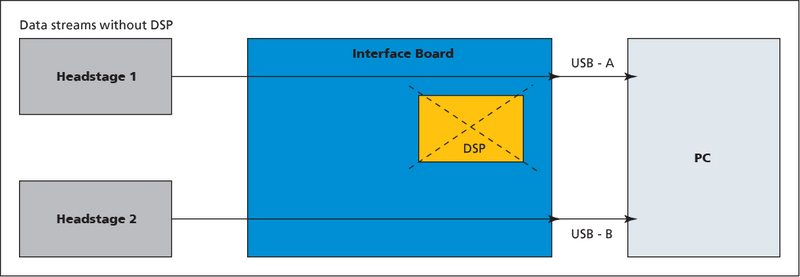
\includegraphics[width=\linewidth]{images/regular_operation.png}
    \caption{Casual mode}
    \label{fig:IFB_regular}
\end{figure}
\begin{figure}[h!]
    %\centering
    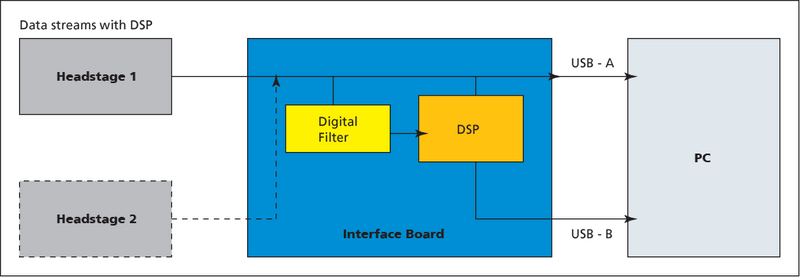
\includegraphics[width=\linewidth]{images/dsp_operation.png}
    \caption{DSP active}
    \label{fig:IFB_DSP}
\end{figure}
\begin{figure}[h!]
    %\centering
    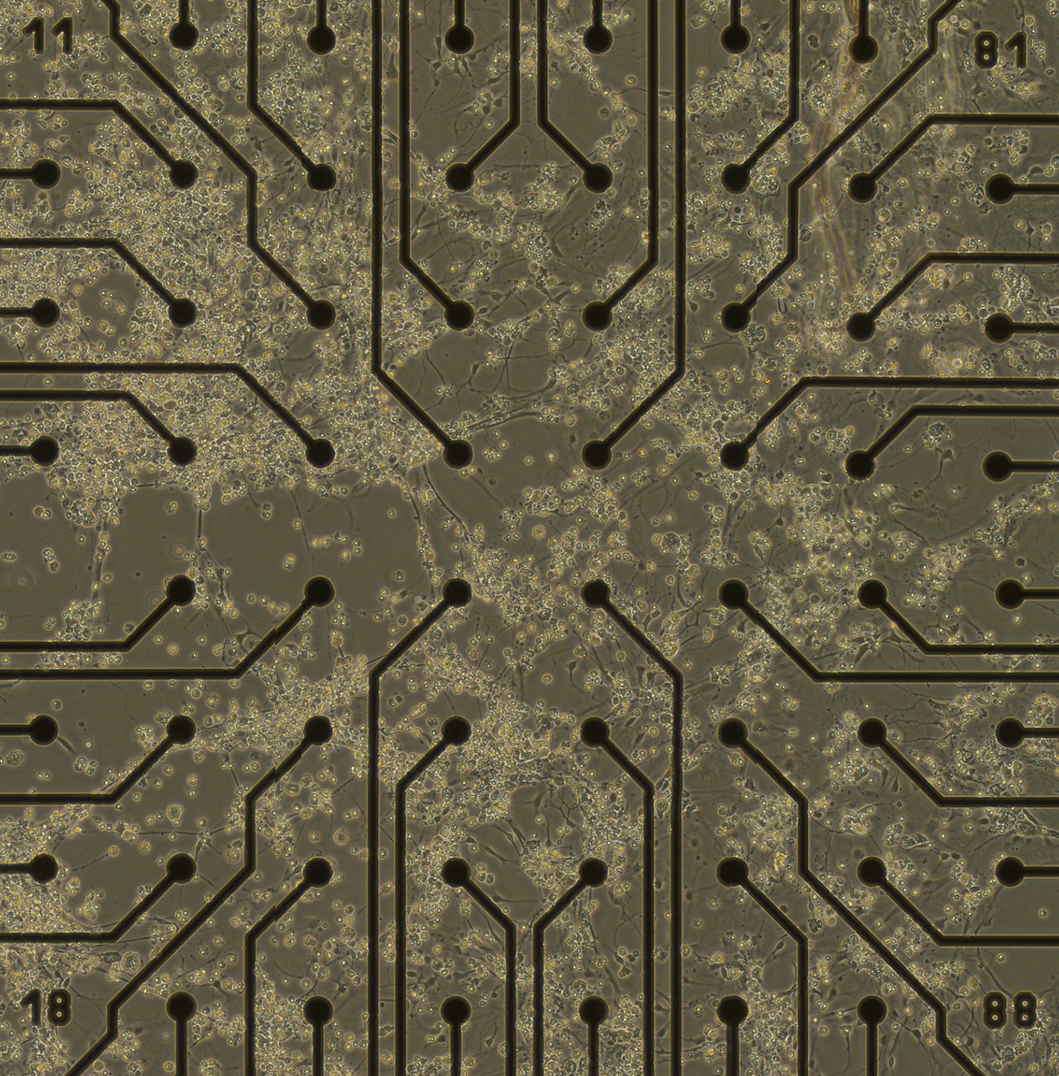
\includegraphics[width=\linewidth]{images/cells.png}
    \caption{Microscopic image on neural networks with visible structures}
    \label{fig:cellular_networks}
\end{figure}
\begin{figure}[h!]
    %\centering
    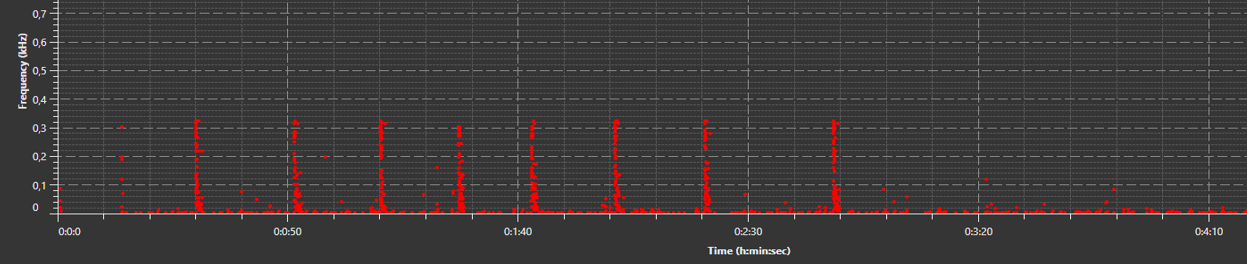
\includegraphics[width=\linewidth]{images/crop_corr28.png}
    \caption{A recording of spikes in a neural culture. Readings performed by
      Ola Huse Ramstad at the department of neuroscience}
    \label{fig:pacemaker}
\end{figure}
\begin{figure}[h!]
    %\centering
    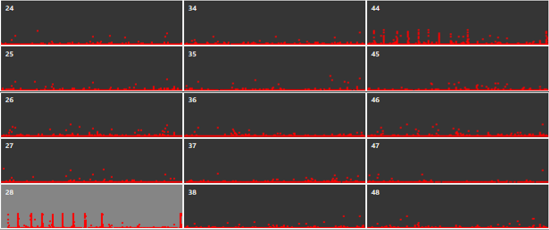
\includegraphics[width=\linewidth]{images/tonic1.png}
    \caption{The grayed out cell in the bottom left shows the readouts in
      \ref{fig:pacemaker}.
      Each cell corresponds to one of the electrodes as seen in
      \ref{fig:cellular_networks}. Even though electrode 28 and electrode 44 are
      far away from each other there seems to be a clear correlation between these two
    sites.}
    \label{fig:correlation}
\end{figure}
\begin{figure}[h!]
    %\centering
    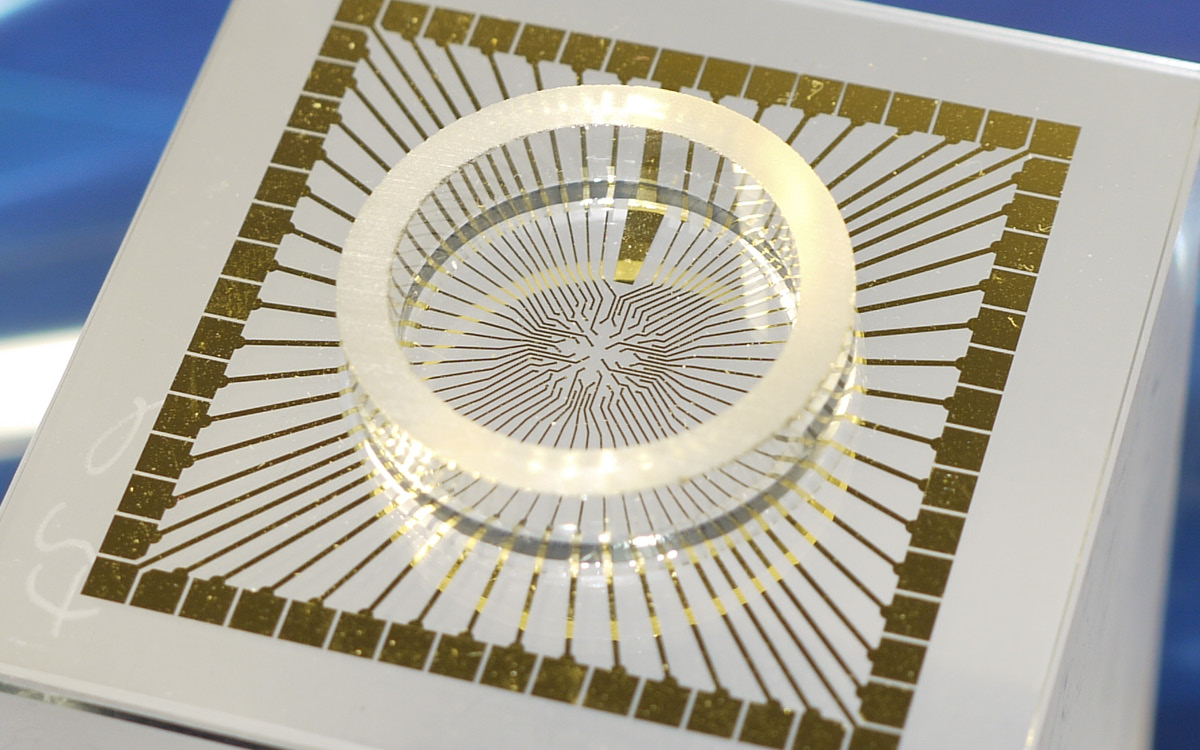
\includegraphics[width=\linewidth]{images/MEA.jpg}
    \caption{A generic MEA}
    \label{fig:generic_MEA}
\end{figure}

\begin{figure}[h!]
    %\centering
    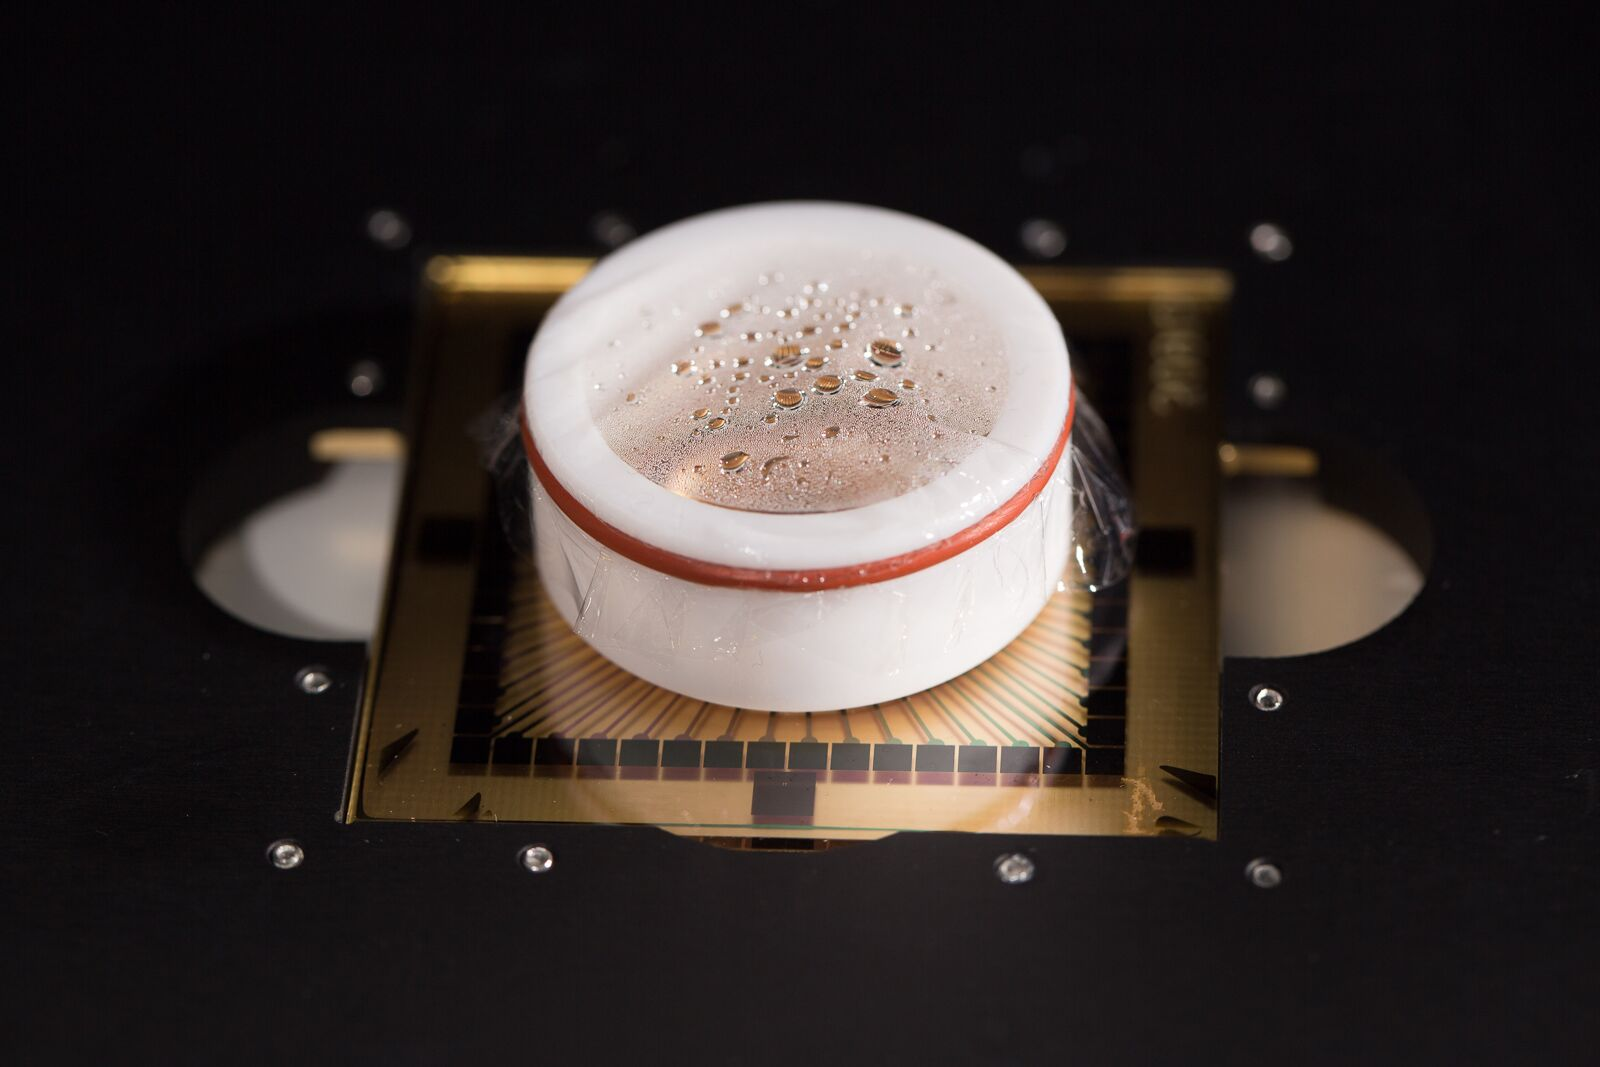
\includegraphics[width=\linewidth]{images/st-olavs-mea.jpg}
    \caption{A MEA with a live culture, photographed by Kai}
    \label{fig:st_olav_MEA}
\end{figure}
\begin{figure}[h!]
    %\centering
    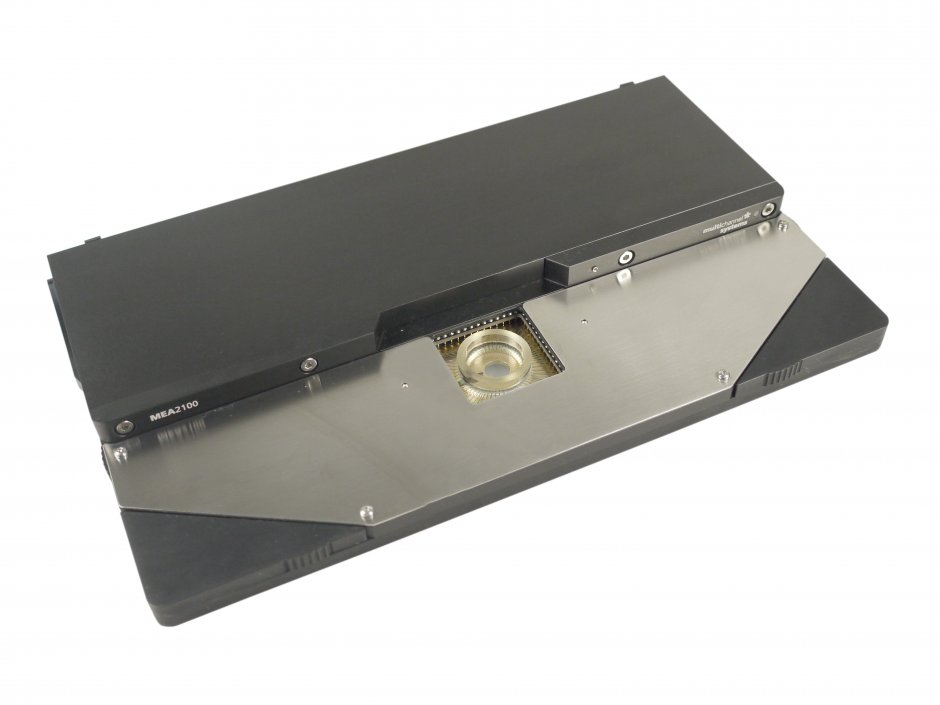
\includegraphics[width=\linewidth]{images/MEA2100-HS60.jpg}
    \caption{The headstage}
    \label{fig:headstage}
\end{figure}
\begin{figure}[h!]
    %\centering
    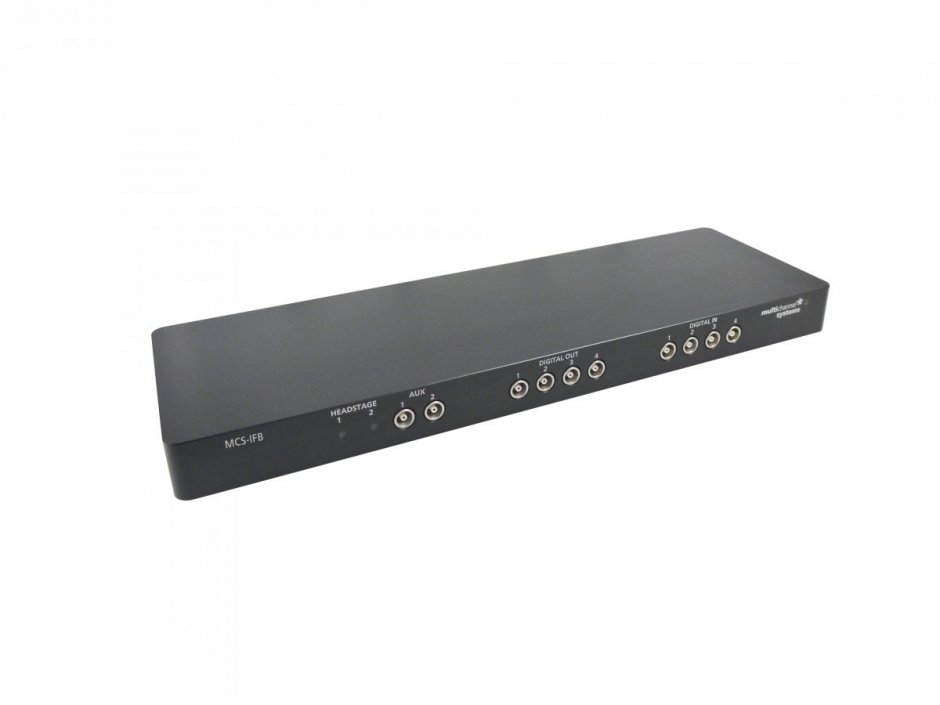
\includegraphics[width=\linewidth]{images/MCS-IFB.jpg}
    \caption{The MCS interface board}
    \label{fig:neuron_anatomy}
\end{figure}
%%% Local Variables:
%%% mode: latex
%%% TeX-master: "../main"
%%% End:
